\documentclass{scrartcl}
\newcommand{\frontorbackendtype}{Frontend}
\hyphenation{
	Ab-bil-dung
	Ab-kür-zung
	Ab-schnitt
	Ac-count
	Ac-counts
	Ad-mi-nis-t-ra-ti-on
	Ad-mi-nis-t-ra-to-ren
	Ad-mi-nis-t-ra-tor
	Ad-res-se
	Ad-res-sen
	Al-len
	Al-ler
	Al-ter
	An-fra-ge
	An-fra-gen
	An-lie-gen
	An-lie-gens
	An-mel-dung
	An-sicht
	An-wen-dung
	An-zahl
	An-zei-gen
	Ant-wor-ten
	Ant-wort
	Apa-che
	Ar-beits-spei-cher
	Ar-ten
	Auf-bau
	Auf-ru-fen
	Auf-tau-chen
	Aus-nah-me
	Aus-wahl-box
	Be-dürf-nis-se
	Be-fin-den
	Be-gin-nen
	Be-grün-dung
	Be-nut-zer
	Be-nut-zers
	Be-nut-zung
	Be-rei-che
	Be-rich-te
	Be-schrei-bung
	Be-zeich-nung
	Bei-spiel
	Book-mark
	But-tons
	Da-ten-bank
	De-tails
	Do-ku-ment
	Do-zent
	Ein-füh-rung
	Ein-lei-tung
	Ein-stel-lung
	Ein-trag
	Er-stel-lung
	Ers-tem
	Feh-ler-be-he-bung
	Fein-des-hand
	Fest-le-gung
	For-mat
	Funk-ti-o-nen
	Ge-bäu-den
	Ge-bäu-des
	Ge-heim-hal-tung
	Goo-gle
	Ha-kens
	Hei-rat
	Ih-rem
	In-for-ma-ti-o-nen
	In-s-ti-tu-tes
	In-s-ti-tut
	Klar-text
	Klo-nen
	Kon-takt
	Kon-ven-ti-o-nen
	Letz-tem
	Mo-dul
	Nie-mand
	Nor-bert
	Nor-ma-li-sie-rung
	Ober-flä-che
	Obers-ten
	Pass-wort
	Pla-nung
	Pro-b-le-me
	Prü-fung
	Samm-lung
	Schrift-art
	Se-kun-den-takt
	Se-mes-ters
	Sei-ten-rand
	Stu-di-en-gan-ges
	Stu-di-en-gang
	Stu-di-ums
	Sys-tem
	Ver-an-stal-tung
	Ver-bin-dung
	Ver-fü-gung
	Ver-knüp-fung
	Ver-wal-tung
	Vor-gang
	Vor-le-sung
	Zen-t-ra-len
	Zu-griff
	Zu-ord-nung
	Zu-satz-in-for-ma-ti-o-nen
	ab-ge-legt
	ab-s-t-rak-te
	ab-s-t-rak-ter
	ab-sol-viert
	ad-mi-ni-s-tra-tor
	ad-mi-ni-stra-tion
	ad-ress-en
	adres-se
	ak-tu-el-lem
	ak-tu-ell
	ak-zep-tiert
	al-le-samt
	an-ge-legt
	an-ge-mel-det
	an-ge-zeigt
	ant-wort
	aus-ge-führt
	aus-ge-füllt
	aus-ge-wählt
	aus-wählt
	ba-ckend
	ba-siert
	bar-ri-e-re-frei-es
	bar-ri-e-re-freie
	be-ant-wor-tet
	be-ar-bei-tet
	be-fin-det
	be-han-delt
	be-in-hal-tet
	be-kommt
	be-legt
	be-lie-big
	be-nutzt
	be-ste-hen
	be-ste-hend
	be-steht
	be-vor-zugt
	bie-tet
	ca-chen
	check-box
	da-bei
	da-für
	da-ge-gen
	da-nach
	da-r-auf
	da-r-um
	def-in-ition
	di-rekt
	die-sem
	do-ku-ment
	drin-gend
	edi-tie-ren
	ei-nem
	ein-ge-pflegt
	ein-ge-schränkt
	ein-ma-lig
	ent-fernt
	ent-hält
	er-bracht
	er-hält
	er-laubt
	er-le-digt
	er-scheint
	er-schwert
	er-stellt
	ers-tem
	even-tu-ell
	ex-akt
	fer-tig
	fest-ge-legt
	fin-det
	frei-ge-schal-tet
	funk-ti-o-niert
	ganz-tä-gig
	ge-fil-tert
	ge-fragt
	ge-langt
	ge-loggt
	ge-löscht
	ge-macht
	ge-mel-det
	ge-nannt
	ge-ne-riert
	ge-nutzt
	ge-nü-gend
	ge-ord-net
	ge-plant
	ge-sagt
	ge-schieht
	ge-sen-det
	ge-setzt
	ge-spei-chert
	ge-sucht
	ge-wählt
	ge-währt
	ge-än-dert
	ge-öff-net
	goo-gle
	gräu-li-che-rem
	halb-wegs
	her-ge-stellt
	hi-e-r-ar-chi-scher
	hi-e-r-ar-chisch
	hin-zu-ge-fügt
	häu-fig
	ih-rem
	in-sti-tut
	in-sti-tute
	in-te-r-es-siert
	je-dem
	je-mand
	kei-ne
	kei-nen
	klo-nen
	kom-pe-tent
	kon-sis-tent
	kon-takt
	ku-rze
	lei-tet
	letz-tem
	lis-tet
	ma-nu-ell
	min-des-tens
	mit-ge-teilt
	mod-ule
	na-vi-ga-tion
	nie-mand
	not-wen-dig
	nö-tig
	obe-ren
	obers-ten
	on-li-ne
	op-tion-al
	per-sis-tent
	plan-en
	po-ten-zi-ell
	re-a-len
	re-d-un-dan-ten
	re-la-tiv
	re-le-vant
	run-ter
	sei-nen
	sie-he
	sim-plic-ity
	so-fort
	spe-zi-ell
	spei-chert
	stu-dent-en
	stu-dium
	sys-tem
	trotz-dem
	un-ab-hän-gig
	un-nö-tig
	un-ter-punkt
	un-ter-wegs
	up-da-ten
	ver-birgt
	ver-hin-dert
	ver-knüpft
	ver-linkt
	ver-sam-melt
	ver-schwin-det
	ver-wal-tet
	voll-stän-dig
	weit-ge-hend
	wel-chem
	zen-t-ra-len
	zen-t-ral
	zu-fäl-lig
	zu-ge-ord-net
	zu-ge-sagt
	zu-griff
	zu-sam-men-ge-führt
	Än-de-rung
	Über-sicht
	über-all
	über-prüft
        Ab-kür-zung
        Ab-schnitt
        Ac-count
        Ac-counts
        Ad-mi-nis-t-ra-ti-on
        Ad-mi-nis-t-ra-to-ren
        Ad-mi-nis-t-ra-tor
        Al-len
        Al-ler
        Al-ter
        An-fra-ge
        An-fra-gen
        An-lie-gen
        An-lie-gens
        An-mel-dung
        An-sicht
        An-zahl
        An-zei-gen
        Ant-wor-ten
        Apa-che
        Ar-beits-spei-cher
        Ar-ten
        Auf-bau
        Auf-ru-fen
        Auf-tau-chen
        Aus-nah-me
        Be-dürf-nis-se
        Be-fin-den
        Be-gin-nen
        Be-grün-dung
        Be-nut-zer
        Be-nut-zers
        Be-nut-zung
        Be-rei-che
        Be-rich-te
        Bei-spiel
}


\usepackage{mathtools}
\usepackage{fontawesome}
\usepackage{amsmath}
\usepackage{titlesec}
\usepackage{float}
\usepackage{tikz}
\usepackage{graphicx}
\usepackage[
	citestyle=authortitle-ibid,
	isbn=true,
	url=true,
	backref=true,
	backrefstyle=none,
	pagetracker=true,
	maxbibnames=50,
	defernumbers=true,
	maxcitenames=10,
	backend=bibtex,
	urldate=comp,
	dateabbrev=false,
	sorting=nty,
	ibidtracker=true
]{biblatex}
\bibliography{literatur.bib}
\usepackage{MnSymbol,wasysym}

\usepackage[T1]{fontenc}
\usepackage[utf8]{inputenc}
\usepackage[ngerman]{babel}
\usepackage{wallpaper}
\usepackage{hologo}
\usepackage{manfnt}
\usepackage{scrextend}
\usepackage{framed,color,verbatim}
\definecolor{shadecolor}{rgb}{.9, .9, .9}

\usepackage{polyglossia}
\setmainlanguage[babelshorthands=true]{german}
\usepackage{enumitem}
\setitemize{itemsep=0pt}


\usepackage{eulervm}
\usepackage{beton}
\usepackage{noto}
\usepackage{fontspec}
\usepackage{xltxtra}
\usepackage{xunicode}
\usepackage{fixltx2e}
\usepackage{xunicode}
\defaultfontfeatures{Mapping=tex-text}

\usepackage{url}
\makeatletter
\g@addto@macro{\UrlBreaks}{\UrlOrds}
\makeatother

\usepackage{color}   %May be necessary if you want to color links
\usepackage{hyperref}
\hypersetup{
	    colorlinks=false, %set true if you want colored links
	    linktoc=all,     %set to all if you want both sections and subsections linked
	    linkcolor=blue,  %choose some color if you want links to stand out
	    hidelinks
}

\emergencystretch2em
\usepackage{longtable}
\usepackage{etoolbox}

\newcommand{\centeredquote}[2]{
	\hbadness=5000
	\vspace{-1em}
	\begin{flushright}
		\item\frqq\textsl{#1}\flqq\ 
	\end{flushright}
	\nopagebreak
	\hfill ---\,\textsc{#2}\newline
	\vspace{-1em}
}



\newcommand{\dollar}{}
\newcommand{\mydbend}{{\textdbend}}

\usepackage{endnotes}
\let\footnote=\endnote

\newenvironment{technisches}{\par\medskip\snugshade\begingroup\begin{addmargin}[2em]{0em}\mydbend\ }{\end{addmargin}\endgroup\medskip\endsnugshade}

\title{Dokumentation zum \frontorbackendtype\ des VVZs}
\author{Norman Koch}

\setcounter{secnumdepth}{6}

\titleclass{\subsubsubsection}{straight}[\subsection]

\newcounter{subsubsubsection}[subsubsection]
\renewcommand\thesubsubsubsection{\thesubsubsection.\arabic{subsubsubsection}}
\renewcommand\theparagraph{\thesubsubsubsection.\arabic{paragraph}} % optional; useful if paragraphs are to be numbered

\titleformat{\subsubsubsection}
  {\normalfont\normalsize\bfseries}{\thesubsubsubsection}{1em}{}
  \titlespacing*{\subsubsubsection}
  {0pt}{3.25ex plus 1ex minus .2ex}{1.5ex plus .2ex}

  \makeatletter
  \renewcommand\paragraph{\@startsection{paragraph}{5}{\z@}%
    {3.25ex \@plus1ex \@minus.2ex}%
      {-1em}%
        {\normalfont\normalsize\bfseries}}
	\renewcommand\subparagraph{\@startsection{subparagraph}{6}{\parindent}%
	  {3.25ex \@plus1ex \@minus .2ex}%
	    {-1em}%
	      {\normalfont\normalsize\bfseries}}
	      \def\toclevel@subsubsubsection{4}
	      \def\toclevel@paragraph{5}
	      \def\toclevel@paragraph{6}
	      \def\l@subsubsubsection{\@dottedtocline{4}{7em}{4em}}
	      \def\l@paragraph{\@dottedtocline{5}{10em}{5em}}
	      \def\l@subparagraph{\@dottedtocline{6}{14em}{6em}}
	      \makeatother

	      \setcounter{secnumdepth}{5}
	      \setcounter{tocdepth}{5}

%\linespread{1.16}


\newcommand{\ExternalLink}{%
    \tikz[x=1.2ex, y=1.2ex, baseline=-0.05ex]{% 
        \begin{scope}[x=1ex, y=1ex]
            \clip (-0.1,-0.1) 
                --++ (-0, 1.2) 
                --++ (0.6, 0) 
                --++ (0, -0.6) 
                --++ (0.6, 0) 
                --++ (0, -1);
            \path[draw, 
                line width = 0.5, 
                rounded corners=0.5] 
                (0,0) rectangle (1,1);
        \end{scope}
        \path[draw, line width = 0.5] (0.5, 0.5) 
            -- (1, 1);
        \path[draw, line width = 0.5] (0.6, 1) 
            -- (1, 1) -- (1, 0.6);
        }
}

\newcommand*{\fullref}[1]{\hyperref[{#1}]{%\autoref*{#1}
\ExternalLink\textit{\nameref*{#1}} (\ref{#1})}} % One single link

%\linespread{1.2}%
%\selectfont

\begin{document}

\LRCornerWallPaper{1}{bg.jpg}

\maketitle\nocite{raffael}
\thispagestyle{empty}

\newpage
\ClearWallPaper

\tableofcontents

\newpage

\thispagestyle{empty}
\centeredquote{Jede gute Software wird von einem Entwickler geschrieben, der ein persönliches Problem lösen will.}{Eric S. Raymond\footfullcite{kathedralewiki}}

\newpage

\section{Typographische Konventionen}
\label{typographie}

\begin{technisches}
Sehr technische oder abstrakte Erklärungen, die nicht gelesen werden müssen, um die Software
normal zu benutzen, werden mit dem Symbol \frq \mydbend\flq\ gekennzeichnet. Außerdem sind solche
Bereiche grau hinterlegt, um sie optisch hervorzuheben.
\end{technisches}

Verweise auf andere Sektionen werden mit einem \ExternalLink-Zeichen gekennzeichnet, kursiv geschrieben
und mit der Sektionsnummer versehen. In der PDF sind sie außerdem anklickbar und verlinken direkt auf
den referenzierten Verweis. Beispiel: \fullref{typographie}.

Die gesamte Dokumentation wurde mit \XeLaTeX\ in der Schriftart \frq Noto\flq\ gesetzt.

\section{Einleitung}

Die Vorlesungsverzeichnissoftware \frq VVZ\flq\ (von \textbf{V}orlesungs\textbf{v}er\textbf{z}eichnis)
versammelt an einem zentralen Ort alle
für die Planung des Studiums notwendigen Daten. Mit ihm ist es möglich, herauszufinden,
wann wo welche Veranstaltung stattfindet, sich einen Stundenplan zu erstellen und die 
Termine automatisch in den digitalen Kalender einzutragen.

\section{Zu den Cookies}

\begin{technisches}
Cookies sind kleine Textdateien, die auf Ihrem Rechner gespeichert und beim Aufrufen des VVZs an den
VVZ-Server gesendet werden. In diesen sind dann Informationen wie ausgewählte Prüfungsleistungen, Anmeldedaten
für den Administrationsbereich oder ausgewählte Veranstaltungen befinden. Das VVZ nutzt diese Daten nicht, um
Sie zu verfolgen und diese werden auch nirgendwo sonst preisgegeben oder von der Serverseite gespeichert.
Lediglich beim Aufrufen der Seite sind die Cookies im Arbeitsspeicher des Servers, um die Anfrage
bearbeiten zu können.

Die Seite ist auch ohne Cookies weitgehend benutzbar, aber Funktionen wie das Anmelden im Administrationsbereich,
Speichern von Veranstaltungen oder Prüfungsleistungen benötigen Cookies zum Funktionieren.
\end{technisches}




\section{Benutzung und Details}

\begin{figure}[H]
	\centering
	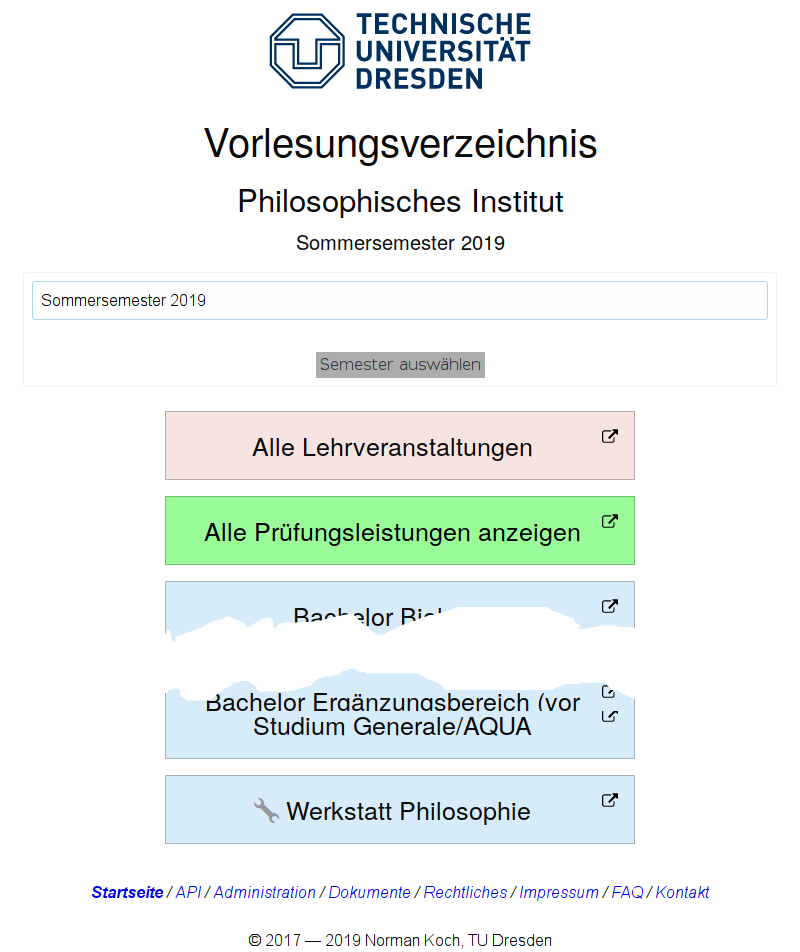
\includegraphics[width=0.9\textwidth]{seite.jpg}
	\caption{Startseite des VVZs}
	\label{startseitefig}
\end{figure}

Auf der Startseite (siehe Abbildung \fullref{startseitefig}) befindet sich eine Auswahlbox mit dem Semester, 
für das die Veranstaltungen
angezeigt werden sollen. Sofern das VVZ mehrere Institute verwaltet, ist dort auch das Institut
auswählbar. Darunter befinden sich alle angebotenen Studiengänge, ein Menü, in dem alle Veranstaltungen
-- unabhängig vom Studiengang -- angezeigt werden und ein Menü, in dem alle Prüfungsleistungen 
angezeigt werden, die am Institut überhaupt möglich sind. 

Ganz unten befinden sich Links zum Impressum, zur Administrationsseite, zur API (siehe \fullref{api}),
zu einem Dokumentenersteller (vgl. \fullref{dokumentenersteller}) und FAQ (vgl. \fullref{faq}).

\subsection{Alle Prüfungsleistungen}

\label{allepls}


\begin{figure}[H]
	\centering
	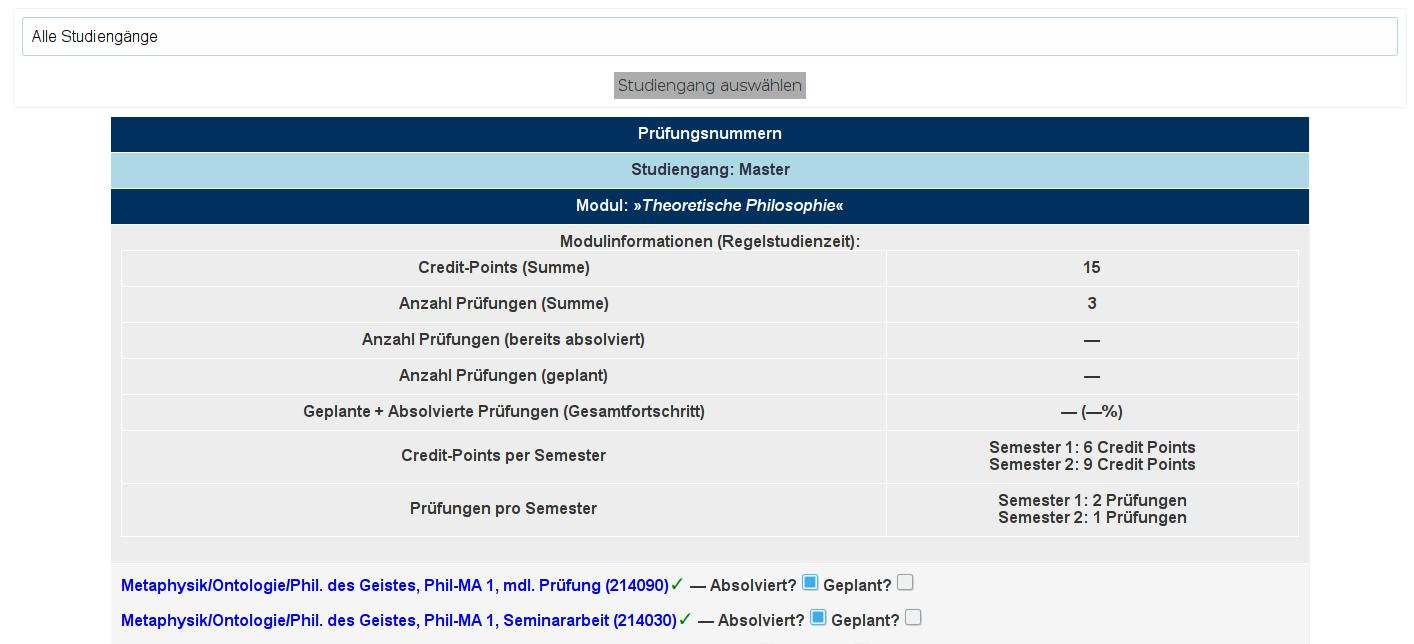
\includegraphics[width=0.9\textwidth]{allepls.jpg}
	\caption{Übersicht aller Prüfungsleistungen}
	\label{alleplsfig}
\end{figure}


Im Menü \frq Alle Prüfungsleistungen anzeigen\flq\ befindet sich eine große Tabelle mit allen
Studiengängen und deren Modulen. Sofern im Backend eingetragen auch zu jedem Modul Informationen
zur Studienordnung, wie viele Prüfungsleistungen welcher Art erbracht werden müssen, wie viele
Credit-Points es dafür gibt und wie viele davon man geplant bzw. absolviert hat (siehe \fullref{planungpruefung}).

Standardmäßig werden alle Studiengänge angezeigt, in der Checkbox überhalb der großen Tabelle lassen
sich jedoch auch einzelne Studiengänge auswählen.

Mit einem Klick auf die Prüfungsnummer wird eine Liste aller Veranstaltungen gezeigt, die diese
Prüfungsnummer anbieten. Von dieser Seite aus ist es möglich, seinen Stundenplan zu planen (siehe
\fullref{stundenplanerstellung}).

\subsubsection{Planung von Prüfungsleistungen}

\label{planungpruefung}

Um die Übersicht zu behalten, lassen sich im Unterpunkt \frq Alle Prüfungsleistungen anzeigen\flq\ zu
jeder angebotenen Prüfungsleistungen zwei Informationen speichern (lokal in einem Cookie). Dazu gibt es neben jeder
Prüfungsleistung zwei Checkboxen mit den Texten \frq Absolviert?\flq\ und \frq Geplant?\flq. Werden diese aktiviert,
dann tauchen auf dem jeweiligen Rechner (solange Cookies persistent bleiben) überall auf der Seite, wo eine Prüfungsnummer
auftaucht, entweder ein grüner Haken (erledigt) oder ein Stift (geplant) auf.

Diese können nach der Auswahl, sofern die Seite sich nicht automatisch neu lädt, mit dem Button
\frq Bereits absolvierte Prüfungsleistungen speichern\flq\ am unteren Seitenrand speichern. Hier gibt
es auch den Button \frq Cookie-URL generieren\flq. Dieser erlaubt es, eine URL zu generieren, die, wenn
man sie aufruft, die gespeicherten Prüfungen auch auf anderen Rechnern zur Verfügung stellt, denen man
die URL mitgeteilt hat (z.\,B. eigener Laptop und Desktop-Rechner).


\subsection{Veranstaltungen}


Durch die Verknüpfung von Veranstaltungen zu Prüfungsleistungen lässt sich jede Veranstaltung
(mit ausgewählten Prüfungsleistungen) mindestens einem Studiengang zuordnen. Sollte keine
Prüfungsleistung ausgewählt worden sein, taucht die Veranstaltung aber in \frq Alle Studiengänge\flq\ auf.

Zu den Veranstaltungen gehören alle wichtigen Daten, die notwendig sind, sie in den eigenen Stundenplan
einzutragen.

\begin{technisches}
Auf der Seite eines Studienganges bzw. aller Studiengänge werden Informationen mehrerer 
Instanzierungen abstrakter Objekte zusammengeführt und dargestellt. Die Objekte sind
hierarchisch geordnet und erben voneinander.

Institute bestehen aus:

\begin{itemize}
	\item Einem Namen
\end{itemize}

(Es können je beliebig viele\footnote{Technisch gesehen ist das falsch,
aber das Limit liegt bei $4\,294\,967\,295$ und ist daher
praktisch nicht relevant.} Studiengänge, Module, Prüfungen und Veranstaltungen hinzugefügt werden.)

Studiengänge bestehen aus:

\begin{itemize}
	\item Einer Zuordnung zu einem Institut
	\item Einem Namen
	\item Einer Studienordnungs-URL (optional)
\end{itemize}

Bereiche bestehen aus:

\begin{itemize}
	\item Einem Namen
\end{itemize}


Module bestehen aus:

\begin{itemize}
	\item Einer Studiengangszuordnung (z.\,B. \frq Bachelor Kernbereich\flq)
	\item Einem Namen
	\item Einer Beschreibung (optional)
	\item Einer Abkürzung (optional)
	\item Einer Zuordnung zu einem Studiengang
\end{itemize}


Prüfungen bestehen aus:

\begin{itemize}
	\item Einer Modulzuordnung (z.\,B. \frq Geschichte der Philosophie\flq)
	\item Einer Bereichszuordnung (z.\,B. \frq Philosophie der Antike\flq)
	\item Einem Prüfungstyp (z.\,B. \frq Essay\flq)
	\item Einer Modulabkürzung (z.\,B. \frq PhF-Phil-MG\flq), optional
	\item Einer Prüfungsnummer (z.\,B. \frq 76210\flq), optional
\end{itemize}


Veranstaltungen bestehen aus:

\begin{itemize}
	\item Titel
	\item Dozent
	\item Gebäude, Raum und Zeit
	\item Die Anzahl der Semesterwochenstunden, die diese Veranstaltung belegt (bei
		Veranstaltungen über mehrere Doppelstunden geschätzt!)
	\item Einzelne, nicht regelmäßige Termine
	\item Einer Verknüpfung zwischen in der Veranstaltung ablegbaren Prüfungsleistungen
\end{itemize}
\end{technisches}

\subsubsection{Menüs in einzelnen Studiengängen/allen Veranstaltungen}

Über der Liste Veranstaltungen sind einige Links:

\begin{enumerate}
	\item \label{linkfilter} Filter anzeigen/ausblenden
	\item \label{linkdetails} Details anzeigen/Ausblenden
	\item \label{linkstundenplanerstellung} Stundenplanerstellung (nur bei Studiengängen, bei
		denen im Backend entsprechende Daten eingegeben worden sind)
	\item \label{linkstudienordnung} Studienordnung (nur bei Studiengängen, bei
		denen im Backend entsprechende Daten eingegeben worden sind)
\end{enumerate}

\subsubsubsection{Filter anzeigen/ausblenden}

Gibt die Möglichkeit, die angezeigten Veranstaltungen weiter
einzuschränken. Hier kann nach Modulen, die eine Veranstaltung enthalten muss, Wochentagen,
Dozenten usw. eingeschränkt werden. Hier kann auch nach Worten im Titel der Veranstaltung
gefiltert werden.

\subsubsubsection{Details anzeigen/ausblenden}

Klappt alle \frq Details\flq-Boxen aller Veranstaltungen auf bzw., wenn
sie bereits auf sind, wieder zu.
Zu den Details, die auch durch Klicken eines Details-Buttons an jeder Veranstaltung einzeln
geöffnet werden kann, gehören folgende Informationen:
\begin{itemize}
	\item Einem Kommentar des Dozenten, sofern vorhanden
	\item Den Link zu OPAL, sofern vorhanden
	\item Einer Liste aus allen im ausgewählten Studiengang (bzw. in allen Studiengängen,
		wenn auf der Startseite \frq Alle Studiengängen\flq\ gewählt worden sind),
		geordnet nach Modulen, in denen die Prüfungsleistungen abgelegt werden können.
		Zusätzlich noch Prüfungen, die vorgemerkt oder bereits erledigt sind (vgl. \fullref{allepls})
	\item Einzelne Veranstaltungen und Orte, die nicht regelmäßig stattfinden
\end{itemize}


\subsubsubsection{Stundenplanerstellung}

Die Stundenplanerstellung nutzt speziell dafür im Backend
eingegebene Daten, daher ist es möglich, dass dieser Button nicht in jedem Studiengang auftaucht. Zum Erstellen von Stundenplänen, siehe
\fullref{stundenplanerstellung}

\subsubsection{Manuelle und Halbautomatische Stundenplanerstellung}

\label{stundenplanerstellung}

\subsubsubsection{Manuelle Stundenplanerstellung}

Links überhalb der Veranstaltungen befindet sich eine kleine Checkbox.
Mit diesen Checkboxen kann man auswählen, welche Veranstaltungen man besuchen möchte. Wählt man diese aus,
kann man am unteren Seitenende \frq Aus markierten Veranstaltungen einen Stundenplan erstellen\flq\ oder diese
Veranstaltungen als Cookie setzen. Hat man bereits Veranstaltungscookies gesetzt und möchte die neu
ausgewählten Veranstaltungen der aktuellen Liste hinzufügen, kann man \frq Stundenplancookies updaten\flq\ auswählen.

Wird aus den markierten Veranstaltungen ein Stundenplan erstellt, gelangt man auf eine Seite mit einem Zeitraster
und dadrinnen allen ausgewählten Veranstaltungen, sofern sie verwertbare Daten haben (d.\,h. Zeit und Wochenrhythmus).

In allen Punkten erscheint auch eine symbolische Hand. Klickt man auf diese, kann man die Einträge des Feldes bearbeiten.
Klickt man dann auf \frq Daten absenden\flq\ kann man die Adresse der Seite kopieren und hat \frq für unterwegs\flq\ immer
einen Stundenplan, oder kann sich die Seite als Bookmark oder Lesezeichen setzen. Dabei werden die Daten nicht
gespeichert und sind ohne diese URL nicht zugänglich.

Darunter ist die Möglichkeit, den ausgewählten Stundenplan automatisch als iCal-Datei zu downloaden und somit
in einen digitalen Kalender einzutragen. Außerdem befindet sich darunter eine Liste von Gebäuden, die oben im Stundenplan
vorkommen und die Möglichkeit, den Stundenplan als PDF-Datei zu downloaden (\mydbend\ experimentell!).

\subsubsubsection{Halbautomatische Stundenplanerstellung}

Klickt man auf den Button namens \frq Stundenplan erstellen\flq, kommt die Frage, für welches Semester ein 
Stundenplan erstellt werden soll. Mit einem Klick auf
Weiter werden die laut Studienordnung für diesen Studiengang und dieses Semester empfohlenen Module
angezeigt. Ein weiterer Klick auf \frq Veranstaltungsauswahl anzeigen\flq\ zeigt nun nur noch Veranstaltungen,
die Module und Prüfungsarten beinhalten, die in diesem Semester gemacht werden sollten. Hier muss nun 
manuell ausgewählt werden, welche Veranstaltungen relevant sind. Ab hier läuft es so ab, wie bei der manuellen
Stundenplanerstellung.

\subsubsection{Alle Veranstaltungen und einzelne Studiengänge}

Nach einem Klick auf \frq Alle Veranstaltungen\flq\ bzw. einen einzelnen Studiengang auf der Startseite
wird eine Liste angezeigt, die alle Veranstaltungen (dieses Studienganges) anzeigt. Von hier aus ist
die Stundenplanerstellung (siehe \fullref{stundenplanerstellung}) möglich. 

\begin{figure}[H]
	\centering
	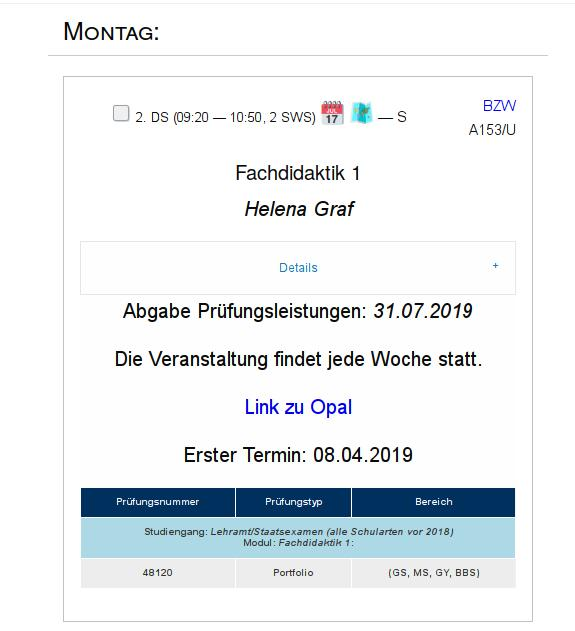
\includegraphics[width=0.9\textwidth]{veranstaltungsbox.jpg}
	\caption{Die Veranstaltungsbox}
	\label{veranstaltungsboxfig}
\end{figure}

\subsubsubsection{Die Veranstaltungsbox (siehe Abbildung \ref{veranstaltungsboxfig})}

Jede einzelne Veranstaltung ist in einer Box dargestellt, die 
Informationen zu ihrer Zeit, ihres Ortes, ihrer Art, ihren Namen, den Namen des Dozenten und einer
Details-Box beinhaltet. Klickt man auf \frq Details anzeigen/ausblenden\flq\ oder auf eine einzelne
Details-Box, sind dort weitere Informationen zu sehen, z.\,B. einen Kommentar des Dozenten, einzelne,
nicht regelmäßige Veranstaltungen und die Prüfungsleistungen, die in dieser Veranstaltung abgelegt
werden können. Bedenken Sie jedoch, dass es oft auch möglich ist, andere Prüfungsleistungen abzulegen als
die Eingetragenen. Fragen Sie dazu einfach mal nett Ihren Dozenten \smiley{}. In der Veranstaltungsbox
befinden sich, sofern der Software die Daten zur Verfügung stehen, etwa in der Mitte oben Buttons zum
Eintragen in den Kalender, ein Link zu Google Earth, wo das Gebäude ist (sehr praktisch mit Google
Street View zum Navigieren) und, rechts hinter dem Gebäudenamen, verbirgt sich ein Link auf die Campusnavigatorseite
des Gebäudes.

\subsubsection{Einzelne Studiengänge}

Die Seiten für alle Veranstaltungen und einzelne Studiengänge unterscheiden sich nur insofern, als dass
in der oberen Leiste für einzelne Studiengänge mehr Informationen auftauchen (z.\,B. die Studienordnung oder
die halbautomatische Stundenplanerstellung, vgl. \fullref{stundenplanerstellung}) und bei den einzelnen
Veranstaltungen in der Details-Box nur noch Prüfungen angezeigt werden, die in diesem Studiengang angeboten
werden können (aus Modulen aus ebendiesem Studiengang).

\subsection{Dokumentenersteller}

\label{dokumentenersteller}

Der halbautomatische Dokumentenersteller ist ein Framework, dass es erlaubt, aus eingegebenen
Daten Dokumente zu befüllen.  Mit einem Klick auf \frq Dokumente\flq\ am
Ende der Seite können Sie Dokumente auswählen, die ausgefüllt werden sollen.
Aktuell ist dort nur das praktischste Dokument des Philosophiestudiums,
\frq Anmeldung zu einer nicht online ausgeschriebenen Prüfung\flq.

Mit einem Klick auf das gewünschte Dokument kommen Sie auf eine Seite zum Eingeben Ihrer Daten.
Aus der Prüfungsnummer wird automatisch das Modul im Dokument eingetragen und Sie erhalten ein
fertig ausgefülltes Dokument, das Sie nur noch unterschreiben und abgeben müssen. Die Daten lassen
sich auch in einem Cookie speichern. 

\subsection{FAQ}

\label{faq}
Der FAQ, kurz für \frq frequently asked questions\flq, enthält einige Links zu wichtigen Studienunterlagen, 
Adressen und Informationen zum Studium.

Wenn Sie im Studium über etwas stolpern, von dem Sie denken, dass es hilfreich wäre, wenn man dieses Wissen
zur Verfügung stellen würde, kontaktieren Sie mich gern und ich trage es ein.

\section{API}

\label{api}

\begin{technisches}
Eine API erlaubt es, Daten in einem einheitlichen Format aus einer Anwendung zu bekommen. Die Daten, die
im Frontend der Software VVZ sind, lassen sich fast allesamt über eine solche API bekommen. Damit ist es
möglich, eigene Anwendungen zu entwickeln, z.\,B. Smartphone-Apps, die auf die Daten des VVZs zugreifen.
\end{technisches}

Zur Benutzung der API, müssen Sie mir eine Email schreiben. Das geht am einfachsten über das Kontaktformular,
das über das untere Ende der Seite aufrufbar ist. Ich teile Ihnen dann einen API-Schlüssel mit, der Sie
berechtigt, auf die Daten des Front-Ends im \frq JSON\flq-Format zuzugreifen. Dieser Schlüssel wird, wenn
er in den Beispielen hier genannt wird, immer \texttt{AUTHKEY} genannt. Sie können die API über einen Browser,
oder über eine HTTPS-Schnittstelle (wie \texttt{wget} oder \texttt{curl}) aufrufen. Eine Beispiel-URL
wäre \url{https://vvz.phil.tu-dresden.de/api.php?auth_code=AUTHKEY&studiengang=1&semester=6}. %$

Folgende Parameter sind möglich:


Achtung: Sie können die API nur einmal pro Sekunde aufrufen. Das ist ein Schutzmechanismus, um den Server
nicht unnötig zu belasten. Am Besten, Sie cachen die Antwort auf Ihrer Seite. Änderungen im VVZ sollten 
sowieso nicht im Sekundentakt passieren.

\noindent\begin{longtable}{l|p{8cm}}
Parameter & Beschreibung\\\hline
\endfirsthead
%
\multicolumn{2}{c}%
{{\bfseries Tabelle von vorheriger Seite\thetable}} \\
\endhead
%
notitle=1 & Ist diese Option nicht gesetzt, sind in der ersten Spalte der JSON-Ausgabe überschriften für die jeweiligen Werte. \\\hline
type=Seminar & Listet nur Veranstaltungen vom Typ Seminar. Mögliche Typen sind: Blockseminar, Exkursion, Fachseminar, Forschungskolloquium, Graduiertenseminar, Hauptseminar, Lesegruppe, Oberseminar, Proseminar, Seminar, Textproseminar, Tutorium, Übung, Vorlesung, Vortrag. \\\hline
gebaeude=BZW & Listet je nur Veranstaltungen in diesem Gebäude. Als Bezeichnung muss die Abkürzung des Gebäudes gewählt werden.\\\hline
gebaeude\_liste=1 & Gibt nur eine Liste aller dem System bekannten Gebäuden der TU Dresden zurück. \\\hline
first\_name=Holm & Sucht nur nach Veranstaltungen, bei dem der Dozent mit erstem Namen Holm heißt. \\\hline
last\_name=Bräuer & Sucht nur nach Veranstaltungen, bei dem der Dozent mit letztem Namen Holm heißt. \\\hline
datetype={[}discordian, unix{]} & Stellt alle Datumsangaben, die vorkommen, auf den diskordianischen bzw. Unix-Kalender um. \\\hline
studiengang=1 & Listet alle Veranstaltungen eines bestimmten Studienganges auf. \\\hline
pruefungen=1 & Listet alle Prüfungen auf, ist kombinierbar mit studiengang=1. \\\hline
semester=1 & Listet Veranstaltungen aus dem Semester 1 auf. \\\hline
institut=1 & Listet Veranstaltungen aus dem Institut 1 auf. \\\hline
institute\_liste=1 & Listet alle Institute auf. \\\hline
semester\_liste=1 & Listet alle Semester auf. \\\hline
studiengang\_liste=1 & Listet alle Studiengänge auf. \\\hline
dozenten\_liste=1 & Listet alle Dozenten auf. \\\hline
veranstaltungstypen=1 & Listet alle Veranstaltungstypen auf.
\end{longtable}

Wenn Sie für Ihre Anwendungen weitere oder andere Daten oder andere Formate benötigen, können Sie uns
jederzeit kontaktieren.

\section{Zukünftige Ideen}

\begin{itemize}
	\item Eigene Stundenpläne erstellen \textit{und} online speichern können
	\item Zentrales Eintragen von Vertretungen, Verspätungen, Verlegungen und Ausfällen,
		dazu -- so gewünscht -- persönliche Email an Studenten, die diese Veranstaltung
		ausgewählt haben
	\item Integration ins OPAL
\end{itemize}

\section{Fehlerbehebung}

Bei gravierenden Fehlern wird automatisch eine Fehlerseite angezeigt und die Administration informiert. 

Kleinere Probleme lassen sich meist selbst beheben. Wenn das Aufklappen von Menüs nicht funktioniert,
aktivieren Sie bitte Javascript. Für die Anmeldung auf der Administrationsseite oder das
Speichern von geplanten/erledigten Prüfungsleistungen oder ausgewählten Veranstaltungen
aktivieren Sie bitte Cookies.

Die Seite sollte in allen halbwegs modernen Browsern funktionieren, inklusive den Konsolenbrowsern \texttt{w3m}
und \texttt{lynx}.

\section{Fehler oder Wünsche melden}

Über den Menüpunkt \frq Kontakt\flq\ ganz unten auf der Seite ist es möglich, mit der Studienberatung oder
mir in Kontakt zu treten. Dazu müssen Sie Ihre Email-Adresse, die Art des Anliegens und das Anliegen selbst
formulieren (die Art des Anliegens bestimmt, wohin die Email geht: bei Technischen Fragen, Wünschen,
Verbesserungsvorschlägen oder Fehlerberichten wählen Sie bitte \frq technischer Natur\flq, sonst
\frq inhaltlicher\flq). Dazu muss gegenenfalls noch eine Sicherheitsabfrage beantwortet werden, die aus
sehr einfachen mathematischen oder geographischen Fragen besteht.

\textit{Jede Email wird gelesen! Es wird um viel Feedback gebeten, da ich die Software so gut wie möglich an
die realen Bedürfnisse von Studenten ausrichten möchte!}

Ich möchte aber darum bitten zu bedenken, dass ich die Software nur als Hobby neben dem Studium betreibe
und daher manchmal etwas länger brauchen kann, um Fehler zu finden oder Wünsche einzubauen.



\section{Urheberrechte \& Danksagungen}

Die Urheberrechte sowohl der Software als auch der Dokumentation liegen bei Norman Koch.

Ich möchte mich außerdem bedanken für die freundliche Hilfe des philosophischen Institutes der Technischen
Universität Dresden, Herrn Prof. Dr. Schönrich,
Herrn Prof. Dr. Rentsch und Herrn Prof. Dr. Hiltscher. Vorallem was das Technische angeht, möchte ich mich für die 
Hilfe von  Herrn Dr. Holm Bräuer und Herrn Norbert Engemaier bedanken.
Auch herzlichen Dank an Frau Gilda Märcz, die mir sowohl im Studium als auch in der Verwaltung
immer sehr freundlich und kompetent geholfen hat.

Ohne die Hilfe, die Bugreports und die freundliche
Art aller Mitarbeiter des Institutes wäre diese Software nie entstanden.

\theendnotes

\section{Quellen}

\DeclareFieldFormat{labelnumberwidth}{---}

\printbibliography[heading=none]

\end{document}

